\documentclass[tikz,border=4pt]{standalone}
% Shared style for every figure and for the deck: one accent, one
% highlight, thin lines, rounded nodes, nothing decorative.
\usepackage[T1]{fontenc}
\usepackage{lmodern}
\renewcommand{\familydefault}{\sfdefault}
\usepackage{tikz}
\usetikzlibrary{arrows.meta,positioning,calc,shapes.misc,fit,backgrounds,decorations.pathreplacing}
\definecolor{ink}{RGB}{40,40,40}
\definecolor{soft}{RGB}{150,150,150}
\definecolor{faint}{RGB}{225,225,225}
\definecolor{accent}{RGB}{0,95,115}
\definecolor{accentlight}{RGB}{214,232,236}
\definecolor{warn}{RGB}{196,84,40}
\definecolor{warnlight}{RGB}{247,226,216}
\tikzset{
  every picture/.style={color=ink, line width=0.5pt, font=\small},
  node distance=12mm and 18mm,
  box/.style={draw=ink, rounded corners=2pt, fill=white, inner sep=5pt, minimum height=7mm, align=center},
  maker/.style={box, minimum width=18mm},
  cat/.style={box, inner sep=3.5pt, minimum height=6mm},
  root/.style={box, fill=accentlight, draw=accent},
  bad/.style={box, fill=warnlight, draw=warn},
  ghost/.style={box, draw=soft, text=soft, dashed},
  flow/.style={-{Stealth[length=4pt,width=3.5pt]}, line width=0.5pt},
  sub/.style={-{Stealth[length=4pt,width=3.5pt]}, line width=0.5pt, color=soft},
  strong/.style={flow, color=accent, line width=0.8pt},
  wrong/.style={flow, color=warn},
  lbl/.style={font=\footnotesize, text=ink, inner sep=1.5pt, fill=white},
  note/.style={font=\footnotesize, text=soft, align=center},
  rate/.style={font=\footnotesize, text=accent, inner sep=1pt, fill=white},
}

\usepackage{amsmath}
\usepackage{pgfplots}
\pgfplotsset{compat=1.17}

\begin{document}
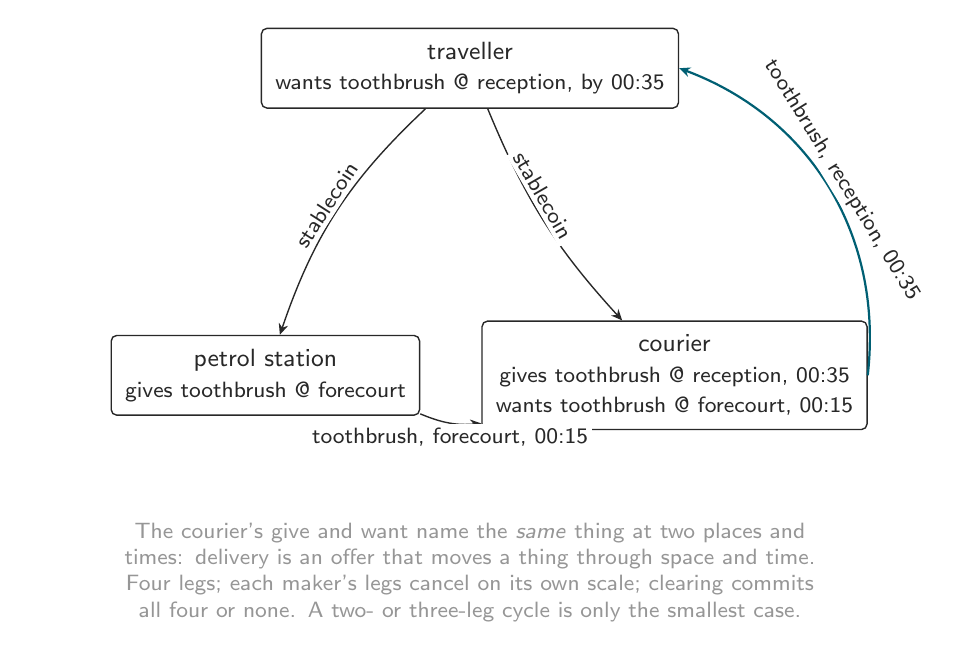
\begin{tikzpicture}
  % A loop with a delivery leg: the courier's offer moves the same thing
  % in place and time. Four legs, three makers; every maker nets to zero
  % on its own scale. A simple cycle is only the smallest case.
  \node[maker, align=center] (T) at (90:24mm) {traveller\\{\footnotesize wants toothbrush @ reception, by 00:35}};
  \node[maker, align=center] (S) at (210:30mm) {petrol station\\{\footnotesize gives toothbrush @ forecourt}};
  \node[maker, align=center] (C) at (-30:30mm) {courier\\{\footnotesize gives toothbrush @ reception, 00:35}\\{\footnotesize wants toothbrush @ forecourt, 00:15}};
  \draw[flow] (T) to[bend right=14] node[lbl, sloped, above] {stablecoin} (S);
  \draw[flow] (T) to[bend right=10] node[lbl, sloped, above, pos=0.4] {stablecoin} (C);
  \draw[flow] (S) to[bend right=14] node[lbl, below] {toothbrush, forecourt, 00:15} (C);
  \draw[strong] (C.east) to[bend right=38] node[lbl, sloped, above, pos=0.5] {toothbrush, reception, 00:35} (T.east);
  \node[note, text width=110mm] at (0,-40mm) {The courier's give and want name the \emph{same} thing at two places and times: delivery is an offer that moves a thing through space and time. Four legs; each maker's legs cancel on its own scale; clearing commits all four or none. A two- or three-leg cycle is only the smallest case.};
\end{tikzpicture}
\end{document}
